\begin{center}
  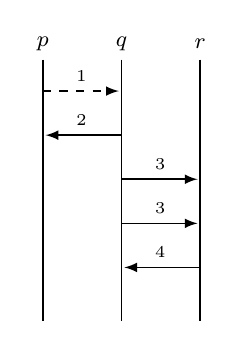
\begin{tikzpicture}[>=stealth,node distance=3.4cm,shorten >=1pt,
  every state/.style={text=black, scale =0.7}, semithick,
    font={\fontsize{8pt}{12}\selectfont}]

\begin{scope}[shift = {(8,0.75)}, scale = 0.8]
%	\draw (0.75, -4) node{\textbf{(b)}};
  %MACHINES
  \draw (0,1.25) node{$q$} ;
  \draw (1.25,1.25) node{$r$} ;
  \draw (-1.25,1.25) node{$p$} ;
  \draw (0,1) -- (0,-3.2) ;
  \draw (1.25,1) -- (1.25,-3.2);
  \draw (-1.25,1) -- (-1.25,-3.2);

  %MESSAGES
  \draw[>=latex,->, dashed] (-1.25, 0.5) -- (0, 0.5) node[ above, midway] {$\amessage_1$};
  \draw[>=latex,->] (0, -0.2) -- (-1.25, -0.2) node[ above, midway] {$\amessage_2$};


  \draw[>=latex,->] (0, -0.9) -- (1.25, -0.9) node[midway, sloped, above] {$\amessage_3$};
  \draw[>=latex,->] (0, -1.6) -- (1.25, -1.6) node[midway, sloped, above] {$\amessage_3$}; %{$\amessage_1'$};
  %\draw[>=latex,->, dashed] (0, -2.5) -- (1.25, -3.25) node[pos=0.55, sloped, above] {$\amessage_1''$};

  %\draw[>=latex,->] (1.25, -0.5) -- (0, -1.75) node[pos=0.1, sloped, above] {$\amessage_4$};
%  \draw[>=latex,->] (1.25, -1.25) -- (0, -2.5) node[pos=0.55, sloped, above] {}; %{$\amessage_2'$};
%  \node[rotate = 90, left]at (1.13, -0.65) {$\cdots$};
%  \node[rotate = -90, right]at (0.1, -0.65) {$\cdots$};

  \draw[>=latex,->] (1.25, -2.3) -- (0, -2.3) node[ above, midway] {$\amessage_4$};


\end{scope}

\end{tikzpicture}
\captionof{figure}{MSC $\mscweakexist$}
\label{fig:msc_weak_exist}
\end{center}
